\section{ENERGY-EFFICIENT POWER BUDGETING FOR MULTI-CORE DARK SILICON SYSTEMS}

Power budgeting, by the name, provides a power budget, which servers as a guidance and constraint for the system. The power budget in dark silicon includes the active cores distribution and their corresponding operating points. Typically, the given power budget should be conservative in order to keep the system in thermally safe state. The energy-efficient power budgeting gives a power budget not only keeps the system thermally safe, but also maximizes the energy efficiency of the system while keeping the power budget as high as possible. 

First, in Section $4.1$, we formulate the energy-efficient power budgeting problem and transforms it into an equivalent problem of minimizing the difference between the chip temperature $T_{c}$ and the target optimal temperature $T_{opt}$. Next, we show how to efficiently calculate the optimal temperature $T_{opt}$ of cores in all positions in Section $4.2$. With the $T_{opt}$, we show how to perform the proposed energy-efficient power budgeting for steady state problem in Section $4.3$, which serves as demonstration for easier understanding of the new method. In Section $4.4$, the full dynamic energy-efficient power budgeting considering transient effects is presented.

\subsection{Power budgeting by minimizing the difference of the chip temperature and the optimal temperature}
The energy-efficient dynamic power budgeting aims to find the optimal active core distribution and their corresponding DVFS stage, which can maximize the PPW of the multi-core system. While some systems may have constraints other than thermal constraint, such as total power supply limit. But the dark silicon systems are extremely thermal limited, therefore, we focus on the major problem of thermal limits, and other constraints can be added with minor modification if needed.

PPW is defined as the ratio of the total performance to the total power.
\begin{equation}\label{eq:ppw}
\text{PPW} = \frac{\left \| f \right \|_{1}}{\left \| P \right \|_{1}}
\end{equation}

For simplicity consideration, the steady state case is presented first, and the energy-efficient power budgeting problem can be formulated as the following optimization problem
\begin{equation}\label{eq:opt_ppw}
\begin{split}
\text{maximize } & PPW = \frac{\left \| f \right \|_{1}}{\left \| P \right \|_{1}}\\
\text{subject to} &\left\{
\begin{array}{lr}
\text{card}(P) = n_{a},\\
T_{c} \preceq T_{th}.\\
\end{array}
\right.
\end{split}
\end{equation}
where $T_{th} \in \mathbb{R}^{n}$ is the temperature rise threshold vector containing the maximum allowed temperature rises from the ambient temperature; card$(P)$ means the cardinality or size of the vector $P$, which is defined as the number of the nonzero components in $P$. In our case, card$(P) = n_{a}$ means there are $n_{a}$ active cores.


\begin{figure}
  \centering
  \subfigure[Temperature distribution of maximized energy efficiency and optimal performance.]{
    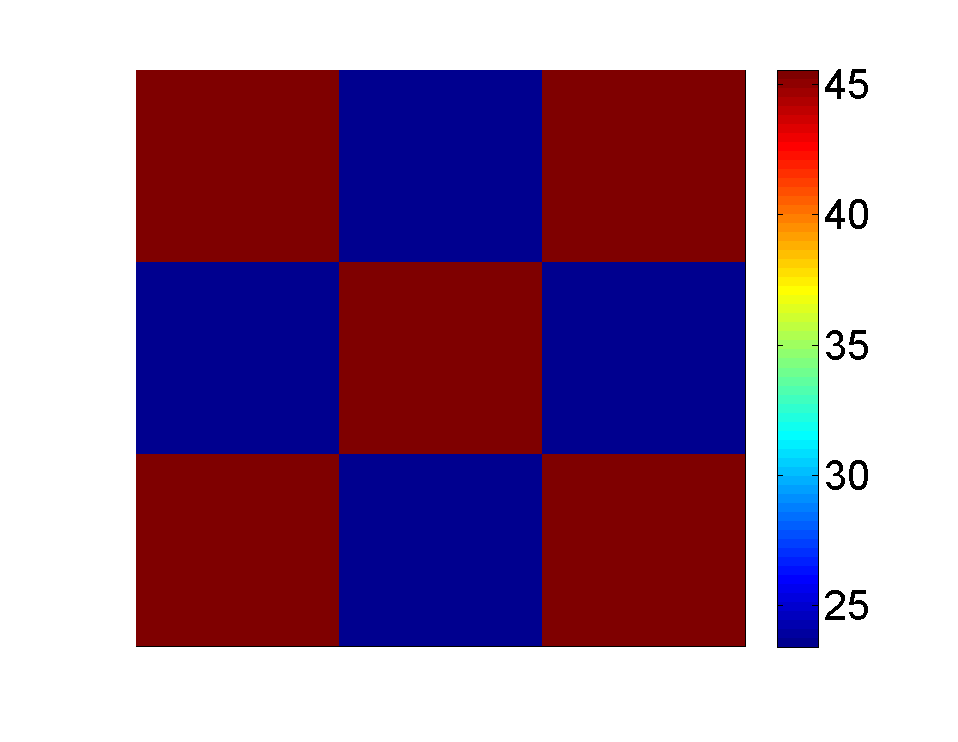
\includegraphics[width=0.46\columnwidth]{fig/opt_tem_1.eps}\label{fig:opt_tem_1}
  }
  \subfigure[Temperature distribution of maximized energy efficiency and worse performance.]{
    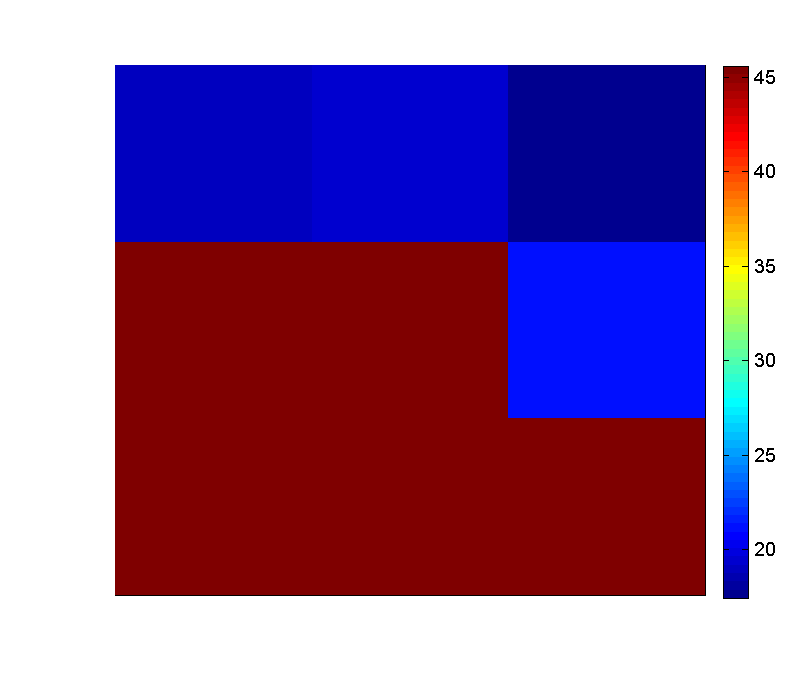
\includegraphics[width=0.46\columnwidth]{fig/opt_tem_2.eps}\label{fig:opt_tem_2}
  }
  \subfigure[Temperature distribution of optimal active cores distribution and random operating points.]{
    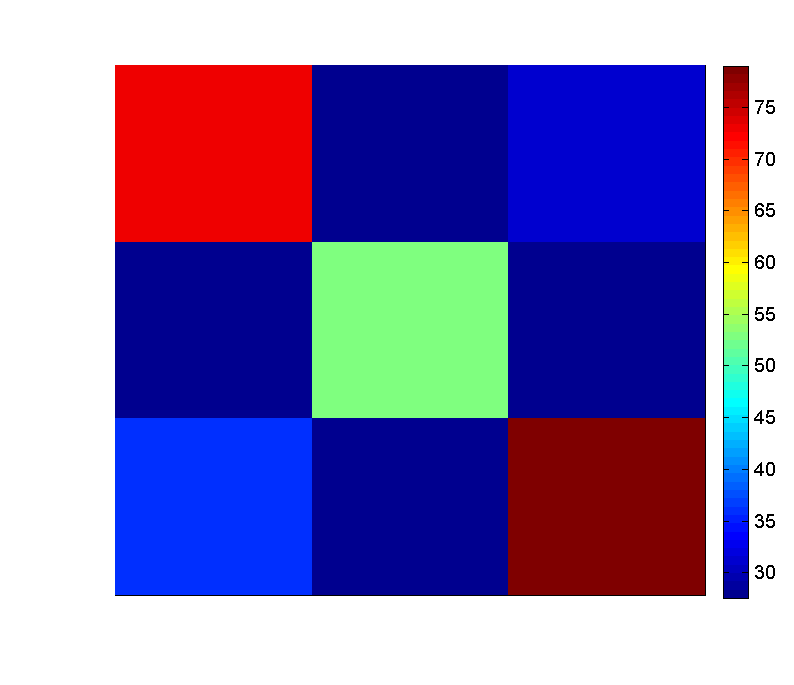
\includegraphics[width=0.46\columnwidth]{fig/opt_tem_3.eps}\label{fig:opt_tem_3}
  }
  \subfigure[Temperature distribution of maximized performance.]{
    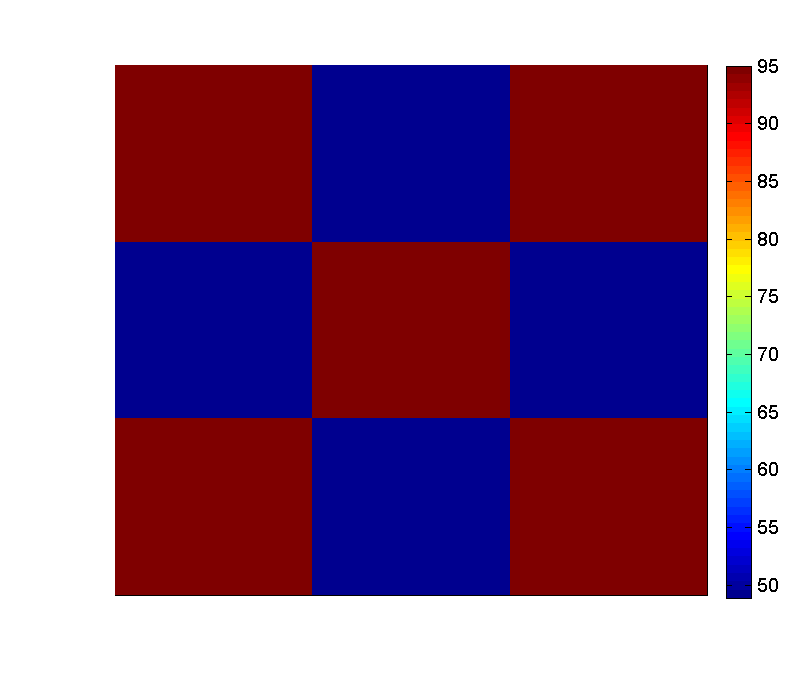
\includegraphics[width=0.46\columnwidth]{fig/opt_tem_4.eps}\label{fig:opt_tem_4}
    }
  \caption{Temperature distributions of a 16-core system with 8 cores active with different power budget.}
  \label{fig:opt_tem}
\end{figure}


The optimization problem in \eqref{eq:opt_ppw} is very hard to solve, because of the high computational complexity of the problem. Therefore, we need to transform this problem into a problem with low complexity. We find out that an optimal temperature vector $T_{opt}$ exists. If a core is running at its corresponding optimal temperature, then the PPW of the core is maximized.

In Fig.~\ref{fig:opt_tem}, the temperature distributions of a $9$-core system with $5$ active cores in different power budget are shown. In Fig.~\ref{fig:opt_tem_1}, the energy efficiency of the system is maximized, the performance of the system is also optimal. In Fig.~\ref{fig:opt_tem_2}, the energy efficiency of the system is also maximized, however, the performance of the system is far worse than optimal. In Fig.~\ref{fig:opt_tem_3}, the active core distribution is the same as Fig.~\ref{fig:opt_tem_1}, however, due to the random operating points of active cores, the energy efficiency is not maximized. Fig.~\ref{fig:opt_tem_4} shows the temperature distribution of the system with maximized performance, yet the energy efficiency of it is also not optimal.

As can be seen in Fig.~\ref{fig:opt_tem}, the maximized PPW of the system can be obtained if all active cores are running at $T_{opt}$. To further maximized the performance of the system while the energy efficiency is optimal, the distribution of active cores needs to be carefully chosen.

Therefore, by minimizing the difference of the core temperature rise $T_{c}$ and the optimal temperature $T_{opt}$, the PPW of the multi-core system can be maximize. In another word, we prefer the power budget induced temperatures of all active cores to be the optimal temperature $T_{opt}$, without violating the thermal constraint.

The optimal temperature vector $T_{opt}$ is actually not a fixed-value vector, it is related to the active core number, and the active core distribution. Also, the optimal temperatures for cores in different positions of the system varies. 

%For the $9$-core system, we can see that there are $3$ unique core positions. We set the active core number to $1$, then we plot the PPW versus the core temperature for each of the $3$ cores in Fig. x. We can see that, as the core temperature rises, the PPW will decrease after reaching a peak value, which means a optimal temperature $T_{opt}$ exists. Also, the $T_{opt}$ for the $3$ cores in different positions varies.

We have shown that the closer the chip's temperature $T_{c}$ is to the optimal temperature $T_{opt}$, the higher the energy efficiency of the system. So instead of directly maximizing PPW, the optimization problem can be transformed to minimizing the difference between $T_{c}$ and $T_{opt}$:
\begin{equation}\label{eq:opt_topt}
\begin{split}
\text{minimize } &  \left \| T_{opt} - T_{c} \right \|_{2}\\
\text{subject to} &\left\{
\begin{array}{lr}
\text{card}(P) = n_{a},\\
T_{c} \preceq T_{th}.\\
\end{array}
\right.
\end{split}
\end{equation}

The optimal temperature $T_{opt}$ needed for the optimization problem in \eqref{eq:opt_topt} is dependent on active core number and active core distribution, which makes it impossible to efficiently calculate the $T_{opt}$ for all senerios, when the core number is high. Fortunately, such problem can be solved efficiently, as shown next.

\subsection{Optimal temperature calculation}
The optimal temperature $T_{opt}$ is relative to many variables, such as active core number, active core distribution and the core's position in the multi-core system. A brute force method to test all possible temperatures for each of the senerios, in order to find the corresponding $T_{opt}$ in which the PPW is maximized is too computationally expensive. Therefore, an efficient method to calculate the $T_{opt}$ needed to slove the optimization problem in \eqref{eq:opt_topt} is proposed in this section.

\subsubsection{Optimal temperature for single core}
Instead of calculating the optimal temperature of all cores at the same time, we choose to calculate the optimal temperature for single core. The reason is that, if each of the active cores is running at maximum PPW, then the PPW of the whole system is certainly maximized. 
We only need to calculate the optimal temperature of cores in the unique position of the multi-core system to achieve the optimal temperature vector for the whole system. Also, by calculating the single core's optimal temperature, other cores' thermal impact can be neglected, which can further simplify the calculation.

The optimal temperature is calculated in steady state. To calculate the steady state temperature rise of the chip, the differential term $C\frac{dT(t)}{dt}$ is neglected in 
\eqref{eq:gt}, leading to
\begin{equation}\label{eq:tc}
T_{c} = B^{T}G^{-1}BP.
\end{equation}
Let $A = B^{T}G^{-1}B \in \mathbb{R}^{m \times m}$ to simplify notation, the simplified 
\eqref{eq:tc} can be expressed as
\begin{equation}\label{sim_tc}
T_{c} = AP.
\end{equation}

Please note that, the $A$ matrix links the core temperature and the power consumption directly, which can be used to find the optimal temperature. The diagonal elements in $A$ can be seen as the corresponding cores' resistance, and the non-diagonal elements in the same row in $A$ serves as the other cores' impact on current core's temperature. Therefore, the diagonal elements can be extracted from $A$ to calculate the core's temperature without other cores' impact. For a specific core $i$, its temperature $T_{i}$ can be computed as:
\begin{equation}\label{eq:t_ap}
\begin{split}
T_{i}&=a_{i} \cdot p\\
&=a_{i}(p_{d}+p_{s})\\
&=a_{i}(p_{d}+v (p_{0}+a_{s}(T_{a}+T_{i})),
\end{split}
\end{equation}
where $a_{i}$ stands for the current core's corresponding diagonal element from $A$, and $T_{a}$ is the ambient temperature.

The optimization object of maximizing PPW can be equivalently transformed to minimizing $\frac{1}{\text{PPW}}$:
\begin{equation}\label{eq:min_ppw}
\text{max PPW}\Longleftrightarrow \text{min } \frac{1}{\text{PPW}},
\end{equation}

\begin{equation}\label{eq:1_ppw}
\begin{split}
&\frac{1}{\text{PPW}}\\
=&\frac{p_{d}+p_{s}}{f}\\
=&\frac{p_{d}+a_{s}(T_{i}+T_{a})+p_{0}}{p_{d}^{1/3}}.
\end{split}
\end{equation}

Integrating \eqref{eq:t_ap} into \eqref{eq:1_ppw}, we have
\begin{equation}\label{eq:full_1_ppw}
\begin{split}
&\frac{1}{\text{PPW}}\\
=&p_{d}^{2/3}+p_{d}^{-1/3}\cdot v(a_{s}(a_{i} \cdot p_{d}+a_{i} \cdot p_{0} \cdot v+v \cdot a_{i} \cdot a_{s} \cdot T_{a})\\
&/(1-v \cdot a_{i} \cdot a_{s})+p_{0})
\end{split}
\end{equation}

Note that in\eqref{eq:full_1_ppw}, the only variable is $p_{d}$. As the form of \eqref{eq:full_1_ppw} suggested, an inflection point for the minimum $\frac{1}{\text{PPW}}$ exists. By finding the inflection point, the minimum $\frac{1}{\text{PPW}}$ and the corresponding $p_{d}$ can be obtained. With the obtained $p_{d}$, the optimal temperature can be calculated with \eqref{eq:t_ap}.

By solving \eqref{eq:full_1_ppw} for each of the uniquely positioned cores, the optimal temperatures vector for all cores can be formed.


\subsubsection{Optimal temperature with temperature compensation}
The above mentioned method calculated the optimal temperature without consideration of other cores' thermal impact, which could cause major error in dark silicon system, where the temperature rise caused by other cores could be higher than the temperature rise caused by the core itself. Therefore, a compensation method to modify the temperature is proposed in this section.

The basic idea of this compensation method is to add a temperature compensation parameter $\lambda$, by multiplying the core's temperature $T_{i}$ with $\lambda$, the core's temperature with other active cores' thermal impact can be obtained with approximation.

Just like optimal temperature $T_{opt}$, for different positioned cores, $\lambda$ is not the same. For core $i$, to obtain its $\lambda$, first we calculate the temperature rise $T_{i}$ from itself with \eqref{eq:t_ap}. Then we generate several random active cores distributions, note that core $i$ is included in active cores. By comparing the averaged temperature rise $T_{avg}$ of core $i$ in the random distributions with $T_{i}$, $\lambda$ can be obtained:
\begin{equation}\label{eq:lambda}
\lambda = \frac{T_{avg}-T_{i}}{T_{i}}.
\end{equation}

However, the temperature rise induced by other cores may vary dramatically, for different active core numbers and various active core distributions. If for a single core, only a single $\lambda$ is used to compensate temperature for all senerios, the error could still be large. In our work, for each core, we implement a $\lambda$ for each active core number to eliminate large error. In another word, for each core, we generate a vector, in which elements are the $\lambda$ for each active core number. By integrating all the vectors, a compensation matrix $\Lambda \in \mathbb{R}^{n \times n}$ is created. $\lambda_{ij}$ in $\Lambda$ stands for the compensation parameter for core $i$ when the active core number is $j$.


By integrating $\lambda$ into \eqref{eq:1_ppw}, we have
\begin{equation}\label{eq:c_full_1_ppw}
\begin{split}
&\frac{1}{\text{PPW}}\\
=&\frac{p_{d}+p_{s}}{f}\\
=&\frac{p_{d}+a_{s} \cdot \lambda(T_{i}+T_{a})+p_{0}}{p_{d}^{1/3}}\\
=&p_{d}^{2/3}+p_{d}^{-1/3}\cdot v(a_{s} ((a_{i} \cdot p_{d}+a_{i} \cdot p_{0} \cdot v+v \cdot a_{i} \cdot a_{s} \cdot T_{a})\\
&/(1-v \cdot a_{i} \cdot a_{s})(1+\lambda)+T_{a})+p_{0})
\end{split}
\end{equation}

By solving \eqref{eq:c_full_1_ppw} for every $\lambda$, the optimal temperature matrix can be obtained, in which $T_{ij}$ stands for the optimal temperature for core $i$ when the active core number is $j$.

\subsection{Energy-efficient power budgeting with optimal performance in steady state}
Now that the optimal temperature for all cores in each active core number is obtained, as long as the active cores' temperature is as close to the corresponding $T_{opt}$ as possible, the energy efficiency of the system is maximized, no matter what active core distribution it may be. However, it's not only energy efficiency we are seeking, the throughput of the system is also an important metric, which are affected by the active core distribution greatly in dark silicon system. Therefore, the goal of our energy-efficient power budgeting is to maximize the throughput while the energy efficiency is maximized.

In \eqref{eq:opt_topt}, we have shown that we can allocate energy-efficient power budget by making the temperature of each core as close to the optimal temperature $T_{opt}$ of itself. However, \eqref{eq:opt_topt} is still a combinational problem, which is very hard to solve. In this section, a steady state example is given to show how to efficiently find a sub-optimal solution using a greedy based method. Please note that, we present our method in steady state mainly for the purpose of clarity.

We plug \eqref{sim_tc} into the optimization problem \eqref{eq:opt_topt} and get
\begin{equation}\label{eq:sim_opt_topt}
\begin{split}
\text{minimize } &  \left \| T_{opt} - AP \right \|_{2}\\
\text{subject to} &\left\{
\begin{array}{lr}
\text{card}(P) = n_{a},\\
AP \preceq T_{th}.\\
\end{array}
\right.
\end{split}
\end{equation}

Finding the optimal solution of such optimization problem requires brute force search of all possible combinations of non-zero positions in $P$ which satisfies $\text{card}(P)=n_{a}$. The high complexity of this method makes it not suitable for multi-core system with large number of cores. It is also noticed that for such systems, finding the optimal solution is not necessary. This is due to the fact that when core number is large, each core takes relatively small area, so there exist many sub-optimal active core distributions which only have slightly larger objective value (measured by cost function) than that of the optimal solution. For example, consider a $25$-core system with $13$ cores active. The optimal solution of such system is shown in xx, and one sub-optimal solution is shown in xx. This is also verified in our experiments by comparing the optimal power budget and the sub-optimal power budget, as shown later.

For a $n$-core system with $n_{a}$ active cores, the basic idea of finding such sub-optimal solution is described as follows: we first find the optimal solution for only one active core. Next, we $fix$ the first active core position determined by the first step, and find the optimal solution of two cores, with the second active core position determined. Please note that although we say "optimal" in the second step, such sulotion is only the optimal solution with the first active core fixed at the position determined by the first step, not the true optimal solution for general two active cores. Similarly, in the $(i+1)$-th step, we look for the optimal solution for $i+1$ active cores with the position of $i$ active cores found in all previous steps remain fixed. By proceeding such strategy for $n_{a}$ steps, we can arrive at a sub-optimal solution for $n_{a}$ active cores.

 show the general iterative steps which are used to find the distribution of $n_{a}$ active cores. Assume we have already fixed the position of $i$ active cores. The power


To demonstrate the greedy based method in details, we begin with finding solution for one active core. The optimization problem for one active core is
\begin{equation}\label{eq:1_sim_opt_topt}
\begin{split}
\text{minimize } &  \left \| T_{opt_1} - AP \right \|_{2}\\
\text{subject to} &\left\{
\begin{array}{lr}
\text{card}(P) = 1,\\
AP \preceq T_{th}.\\
\end{array}
\right.
\end{split}
\end{equation}

%We normalize columns of $A$ to simplify discussions (please note we can reverse such operation on solution $P$ to get the original solution), i.e, for $A = [a_{1},a_{2},...,a_{n}]$, we make $\left \| a_{1} \right \|_{2} = \left \| a_{2} \right \|_{2} =\cdot \cdot \cdot = \left \| a_{n} \right \|_{2} = 1$ without changing their directions.

We have to find a way to determine if one core is superior than the other one, measured by the cost function in \eqref{eq:1_sim_opt_topt}. 



One example of comparing two possible active core positions (the $j$-th core and $k$-th core are took as examples) is shown in Fig.x. By turning on $j$-th core only, the corresponding temperature rise of the chip is $a_{j}p_{j}$, where $p_{j}$ is the $j$-th elements in $P$ which should be determined by solving \eqref{eq:1_sim_opt_topt}. Assume $p_{j}$ is correctly computed, then the $T_{j}$ component (temperature rise at position $j$) of $a_{j}p_{j}$ should be the same as the $T_{opt}$, and $T_{k}$ component of $a_{j}p_{j}$ will be lower than $T_{opt}$. Instead, by turning on the $k$-th core only, the corresponding solved power value $p_{k}$ will heat the chip to $a_{k}p_{k}$, with its $T_{j}$ component being lower than $T_{opt}$ and its $T_{k}$ component just being equal to $T_{opt}$. Between the $j$-th core and $k$-th core, we prefer to turn on the $j$-th core, 


because its cost $\left \| T_{opt}-a_{j}p_{j} \right \|_{2}$ (length of $a_{j}p_{j}-T_{th}$ in xx) in the optimization problem \eqref{eq:1_sim_opt_topt} is smaller than the cost $\left \| T_{opt}-a_{k}p_{k} \right \|_{2}$ of turning on the $k$-th core, as observed in Fig. x. The physical meaning is: by turning on the $j$-th core, the overall system temperature is closer to $T_{opt}$. With all cores' temperature lower than $T_{opt}$, the overall system temperature of turning on the $j$-the core is higher than that of turning on the $k$-th core.

